\documentclass{standalone}
\usepackage[ddmmyyyy]{datetime}

% ------------------------------------------------------------------------------
% Packages
% ------------------------------------------------------------------------------
% Page setting
\usepackage[explicit]{titlesec}
\usepackage{sectsty}
\usepackage{fancyhdr}

% Text options
\usepackage{lmodern}
\usepackage[T1]{fontenc}
\usepackage[utf8]{inputenc}
\usepackage{xspace}

\usepackage{amsfonts}
\usepackage{dsfont}
\usepackage{pifont}

\usepackage[color=myred!50]{todonotes}

% Graphics and colors
\usepackage{graphicx}
\usepackage{import}
\usepackage{graphics}
\usepackage{xcolor}

\definecolor{myred}{RGB}{150,0,0}  
\definecolor{mygreen}{RGB}{0,150,0}
\definecolor{myblue}{RGB}{0, 101, 189}
\definecolor{myyellow}{RGB}{220, 206, 0}
\definecolor{myorange}{RGB}{255, 153, 51}
\definecolor{mycyan}{RGB}{51, 204, 204}
\definecolor{mypurple}{RGB}{204, 0, 153}

\newcommand{\doccol}{\color{myblue}}

% Hyperrefs
\usepackage{hyperref}
\hypersetup{
  pdfusetitle,
  unicode = true,
  bookmarks = true,
  bookmarksnumbered = false,
  bookmarksopen = true,
  breaklinks = false,
  pdfborderstyle = {},
  backref = false,
  colorlinks = true,
  linkcolor = myblue,
  urlcolor = myred,
  citecolor = mygreen,
}

% enumerate and itemize
\usepackage{enumitem}

% Appendix
\usepackage[title, titletoc]{appendix}

% Captions
\usepackage{caption}
\usepackage{subcaption}

\captionsetup[figure]{position = bottom}
\captionsetup[table]{position = bottom}

% Figures

% Tables
\usepackage{booktabs}
\usepackage{nicematrix}

\renewcommand{\arraystretch}{1.5}

% Algorithms
\usepackage{algorithm}
\usepackage{algorithmicx}
\usepackage{algpseudocode}

% Math
\usepackage{amsmath}
\usepackage{amsthm}
\usepackage{amssymb}
\usepackage{mathtools}
\usepackage{nicefrac}
\usepackage{bm}
\usepackage{thmtools}
\usepackage{thm-restate}
\usepackage{optidef}

% Theorems
\usepackage[framemethod=TikZ]{mdframed}
\usepackage{xifthen}

% Tikz and pfgplots
\usepackage{tikz}
\usepackage{pgfplots}
\usepackage{pgfplotstable}

\usetikzlibrary{shapes}
\usetikzlibrary{arrows}
\usetikzlibrary{automata}
\usetikzlibrary{positioning}
\usetikzlibrary{calc}
\usetikzlibrary{intersections}

\pgfplotsset{compat=newest}
\usepgfplotslibrary{groupplots}
\usepgfplotslibrary{fillbetween}

% ------------------------------------------------------------------------------
% Math declarations
% ------------------------------------------------------------------------------
\newcommand{\Brac}[2][r]{%
  \ifx r#1 \left(       #2 \right)       \else
  \ifx c#1 \left\{      #2 \right\}      \else
  \ifx s#1 \left[       #2 \right]       \else
  \ifx v#1 \left\vert   #2 \right\vert   \else
  \ifx a#1 \left\langle #2 \right\rangle \else
  \ifx t#1 \left\lceil  #2 \right\rceil  \else
  \ifx b#1 \left\lfloor #2 \right\rfloor \else
  \ifx n#1 \left\|      #2 \right\|      \else
  \mathrm{Illegal~option}%
  \fi\fi\fi\fi\fi\fi\fi\fi
}

\newcommand{\clip}[4][s]{
  \ifx s#1 \mathrm{clip}_{\Brac[s]{#2,\; #3}}\Brac{#4} \else
  \ifx u#1 \mathrm{clip}_{\left[#2,\; #3\right)}\Brac{#4} \else
  \ifx l#1 \mathrm{clip}_{\left(#2,\; #3\right]}\Brac{#4} \else
  \mathrm{Illegal~option}%
  \fi\fi\fi
}

\newcommand{\yesmark}{\textcolor{mygreen}{\ding{51}}}%
\newcommand{\nomark}{\textcolor{myred}{\ding{55}}}
\newcommand{\good}[1]{\textcolor{mygreen}{#1}}
\newcommand{\bad}[1]{\textcolor{myred}{#1}}

\newcommand{\R}{\mathbb{R}}
\newcommand{\N}{\mathbb{N}}
\newcommand{\X}{\mathbb{X}}
\newcommand{\Xc}{\mathcal{X}}
\newcommand{\D}{\mathcal{D}}

\newcommand{\I}{\mathcal{I}}
\newcommand{\Itil}{\tilde{\mathcal{I}}}
\newcommand{\Ineg}{\I_{-}}
\newcommand{\Ipos}{\I_{+}}

\newcommand{\Imb}{\I_{\text{mb}}}
\newcommand{\Imbneg}{\I_{\text{mb},-}}
\newcommand{\Imbpos}{\I_{\text{mb},+}}

\newcommand{\nall}{n}
\newcommand{\nneg}{n_{-}}
\newcommand{\npos}{n_{+}}
\newcommand{\ntil}{\tilde{n}}

\newcommand{\nmb}{n_{\text{mb}}}
\newcommand{\nmbneg}{n_{\text{mb},-}}
\newcommand{\nmbpos}{n_{\text{mb},+}}

\newcommand{\K}{\mathbb{K}}
\newcommand{\Kall}{\K^{\pm}}
\newcommand{\Kneg}{\K^{-}}

\newcommand{\updateaa}{\Delta_{\alpha,\alpha}}
\newcommand{\updateab}{\Delta_{\alpha,\beta}}
\newcommand{\updatebb}{\Delta_{\beta,\beta}}

\newcommand{\alphak}{\alpha_{\hat{k}}}
\newcommand{\alphal}{\alpha_{\hat{l}}}
\newcommand{\betak}{\beta_{\hat{k}}}
\newcommand{\betal}{\beta_{\hat{l}}}

\newcommand{\norm}[1]{\Brac[n]{#1}}
\newcommand{\abs}[1]{|#1|}
\newcommand{\inner}[2]{\Brac[a]{#1, \; #2}}
\newcommand{\dd}[1]{\mathop{}\!\mathrm{d}#1}
\newcommand{\minimize}[1]{\ifthenelse{\isempty{#1}}{\operatorname*{minimize}\quad}{\operatorname*{minimize}_{#1}\quad}}
\newcommand{\maximize}[1]{\ifthenelse{\isempty{#1}}{\operatorname*{maximize}\quad}{\operatorname*{maximize}_{#1}\quad}}
\newcommand{\st}{\operatorname{subject\ to}}
\newcommand{\argmin}{\operatorname*{argmin}}
\newcommand{\eps}{{\varepsilon}}

\newcommand{\Imin}{I_{\rm mb}}
\newcommand{\Iminh}{I_{\rm mb}^{\rm enh}}
\newcommand{\nmin}{n_{\rm mb}}
\newcommand{\II}{\mathds{1}}
\newcommand{\Iverson}[1]{\mathds{1}_{\Brac[s]{#1}}}

\newcommand{\EE}{\mathbb{E}}
\newcommand{\PP}{\mathbb{P}}
\newcommand{\bias}{\operatorname{bias}}

\newcommand{\Matrix}[1]{\begin{pmatrix} #1 \end{pmatrix}}
\newcommand{\Set}[2]{\Brac[c]{#1 \; \middle\vert \; #2}}
\newcommand{\domain}{\operatorname*{dom}}

\newcommand{\repeatloop}{\texttt{repeat}\xspace}
\newcommand{\forloop}{\texttt{for}\xspace}

\newcommand{\vecab}{\Matrix{\bm{\alpha} \\ \bm{\beta}}}

% models
\newcommand{\AccatTop}{\emph{Accuracy at the Top}\xspace}
\newcommand{\TopPush}{\emph{TopPush}\xspace}
\newcommand{\TopPushK}{\emph{TopPushK}\xspace}
\newcommand{\tauFPL}{{\emph{$\tau$-FPL}}\xspace}
\newcommand{\TopMeanK}{\emph{TopMeanK}\xspace}
\newcommand{\PatMat}{\emph{Pat}\&\emph{Mat}\xspace}
\newcommand{\PatMatNP}{{\emph{Pat}\&\emph{Mat-NP}}\xspace}
\newcommand{\Grill}{\emph{Grill}\xspace}
\newcommand{\GrillNP}{\emph{Grill-NP}\xspace}
\newcommand{\DeepTopPush}{\emph{DeepTopPush}\xspace}
\newcommand{\TFCO}{\emph{TFCO}\xspace}
\newcommand{\APPerf}{\emph{Ap-Perf}\xspace}
\newcommand{\BaseLine}{\emph{BaseLine}\xspace}

% counts and rates
\DeclareMathOperator{\tp}{tp}
\DeclareMathOperator{\tn}{tn}
\DeclareMathOperator{\fp}{fp}
\DeclareMathOperator{\fn}{fn}
\DeclareMathOperator{\tpr}{tpr}
\DeclareMathOperator{\tnr}{tnr}
\DeclareMathOperator{\fpr}{fpr}
\DeclareMathOperator{\fnr}{fnr}

\DeclareMathOperator{\tps}{\overline{tp}}
\DeclareMathOperator{\tns}{\overline{tn}}
\DeclareMathOperator{\fps}{\overline{fp}}
\DeclareMathOperator{\fns}{\overline{fn}}

\DeclareMathOperator{\accuracy}{acc}
\DeclareMathOperator{\baccuracy}{bacc}
\DeclareMathOperator{\precision}{precision}
\DeclareMathOperator{\recall}{recall}
\DeclareMathOperator{\pratrec}{Precision@Recall}
\DeclareMathOperator{\postop}{pos@top}

% ------------------------------------------------------------------------------
% Document
% ------------------------------------------------------------------------------
\tikzstyle{line_node} = [line width=1pt, rounded corners, color=black, ->]
\tikzstyle{line_cv} = [line width=3pt, color=mygreen, line cap=round]

\begin{document}
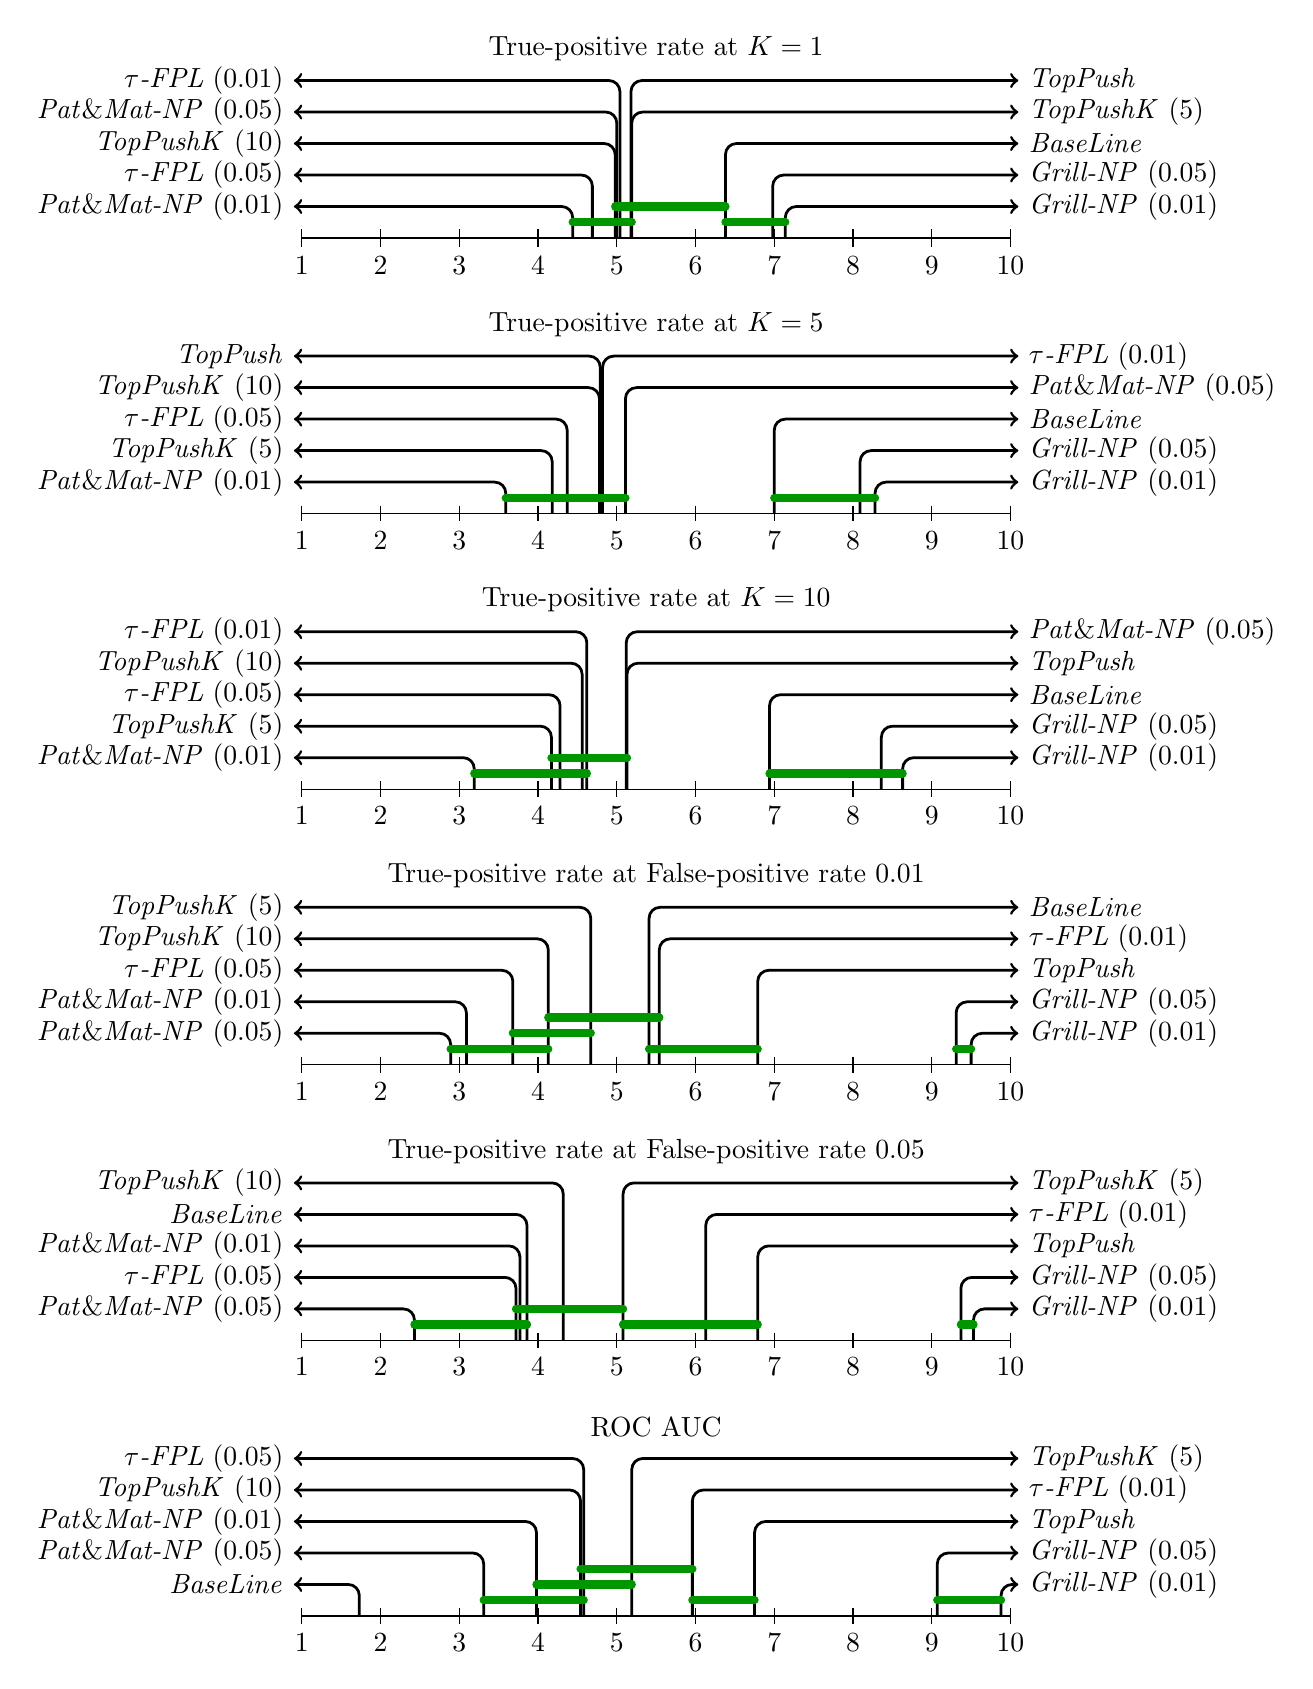
\begin{tikzpicture}
  \node at (5.5,2.4) {ROC AUC}; 
  \draw (1,0) -- (10,0); 
  \foreach \x in {1,...,10} \draw (\x,0.1) -- (\x,-0.1) node[anchor=north]{$\x$}; 
  \draw[line_node] (1.73,0) -- (1.73,0.4) -- (0.9, 0.4) node[anchor=east] {\BaseLine}; 
  \draw[line_node] (3.31,0) -- (3.31,0.8) -- (0.9, 0.8) node[anchor=east] {\PatMatNP(0.05)}; 
  \draw[line_node] (3.98,0) -- (3.98,1.2) -- (0.9, 1.2) node[anchor=east] {\PatMatNP(0.01)}; 
  \draw[line_node] (4.54,0) -- (4.54,1.6) -- (0.9, 1.6) node[anchor=east] {\TopPushK(10)}; 
  \draw[line_node] (4.58,0) -- (4.58,2.0) -- (0.9, 2.0) node[anchor=east] {\tauFPL(0.05)}; 
  \draw[line_node] (5.19,0) -- (5.19,2.0) -- (10.1, 2.0) node[anchor=west] {\TopPushK(5)}; 
  \draw[line_node] (5.96,0) -- (5.96,1.6) -- (10.1, 1.6) node[anchor=west] {\tauFPL(0.01)}; 
  \draw[line_node] (6.75,0) -- (6.75,1.2) -- (10.1, 1.2) node[anchor=west] {\TopPush}; 
  \draw[line_node] (9.07,0) -- (9.07,0.8) -- (10.1, 0.8) node[anchor=west] {\GrillNP(0.05)}; 
  \draw[line_node] (9.88,0) -- (9.88,0.4) -- (10.1, 0.4) node[anchor=west] {\GrillNP(0.01)}; 
  \draw[line_cv] (3.31,0.2) -- (4.58, 0.2); 
  \draw[line_cv] (3.98,0.4) -- (5.19, 0.4); 
  \draw[line_cv] (4.54,0.6) -- (5.96, 0.6); 
  \draw[line_cv] (5.96,0.2) -- (6.75, 0.2); 
  \draw[line_cv] (9.07,0.2) -- (9.88, 0.2); 

  \node at (5.5,5.9) {True-positive rate at False-positive rate $0.05$}; 
  \draw (1,3.5) -- (10,3.5); 
  \foreach \x in {1,...,10} \draw (\x,3.6) -- (\x,3.4) node[anchor=north]{$\x$}; 
  \draw[line_node] (2.43,3.5) -- (2.43,3.9) -- (0.9, 3.9) node[anchor=east] {\PatMatNP(0.05)}; 
  \draw[line_node] (3.72,3.5) -- (3.72,4.3) -- (0.9, 4.3) node[anchor=east] {\tauFPL(0.05)}; 
  \draw[line_node] (3.77,3.5) -- (3.77,4.7) -- (0.9, 4.7) node[anchor=east] {\PatMatNP(0.01)}; 
  \draw[line_node] (3.86,3.5) -- (3.86,5.1) -- (0.9, 5.1) node[anchor=east] {\BaseLine}; 
  \draw[line_node] (4.32,3.5) -- (4.32,5.5) -- (0.9, 5.5) node[anchor=east] {\TopPushK(10)}; 
  \draw[line_node] (5.08,3.5) -- (5.08,5.5) -- (10.1, 5.5) node[anchor=west] {\TopPushK(5)}; 
  \draw[line_node] (6.13,3.5) -- (6.13,5.1) -- (10.1, 5.1) node[anchor=west] {\tauFPL(0.01)}; 
  \draw[line_node] (6.79,3.5) -- (6.79,4.7) -- (10.1, 4.7) node[anchor=west] {\TopPush}; 
  \draw[line_node] (9.37,3.5) -- (9.37,4.3) -- (10.1, 4.3) node[anchor=west] {\GrillNP(0.05)}; 
  \draw[line_node] (9.53,3.5) -- (9.53,3.9) -- (10.1, 3.9) node[anchor=west] {\GrillNP(0.01)}; 
  \draw[line_cv] (2.43,3.7) -- (3.86, 3.7); 
  \draw[line_cv] (3.72,3.9) -- (5.08, 3.9); 
  \draw[line_cv] (5.08,3.7) -- (6.13, 3.7); 
  \draw[line_cv] (6.13,3.7) -- (6.79, 3.7); 
  \draw[line_cv] (9.37,3.7) -- (9.53, 3.7); 

  \node at (5.5,9.4) {True-positive rate at False-positive rate $0.01$}; 
  \draw (1,7.0) -- (10,7.0); 
  \foreach \x in {1,...,10} \draw (\x,7.1) -- (\x,6.9) node[anchor=north]{$\x$}; 
  \draw[line_node] (2.89,7.0) -- (2.89,7.4) -- (0.9, 7.4) node[anchor=east] {\PatMatNP(0.05)}; 
  \draw[line_node] (3.09,7.0) -- (3.09,7.8) -- (0.9, 7.8) node[anchor=east] {\PatMatNP(0.01)}; 
  \draw[line_node] (3.68,7.0) -- (3.68,8.2) -- (0.9, 8.2) node[anchor=east] {\tauFPL(0.05)}; 
  \draw[line_node] (4.13,7.0) -- (4.13,8.6) -- (0.9, 8.6) node[anchor=east] {\TopPushK(10)}; 
  \draw[line_node] (4.67,7.0) -- (4.67,9.0) -- (0.9, 9.0) node[anchor=east] {\TopPushK(5)}; 
  \draw[line_node] (5.41,7.0) -- (5.41,9.0) -- (10.1, 9.0) node[anchor=west] {\BaseLine}; 
  \draw[line_node] (5.54,7.0) -- (5.54,8.6) -- (10.1, 8.6) node[anchor=west] {\tauFPL(0.01)}; 
  \draw[line_node] (6.79,7.0) -- (6.79,8.2) -- (10.1, 8.2) node[anchor=west] {\TopPush}; 
  \draw[line_node] (9.31,7.0) -- (9.31,7.8) -- (10.1, 7.8) node[anchor=west] {\GrillNP(0.05)}; 
  \draw[line_node] (9.5,7.0) -- (9.5,7.4) -- (10.1, 7.4) node[anchor=west] {\GrillNP(0.01)}; 
  \draw[line_cv] (2.89,7.2) -- (4.13, 7.2); 
  \draw[line_cv] (3.68,7.4) -- (4.67, 7.4); 
  \draw[line_cv] (4.13,7.6) -- (5.54, 7.6); 
  \draw[line_cv] (5.41,7.2) -- (6.79, 7.2); 
  \draw[line_cv] (9.31,7.2) -- (9.5, 7.2); 

  \node at (5.5,12.9) {True-positive rate at $K = 10$}; 
  \draw (1,10.5) -- (10,10.5); 
  \foreach \x in {1,...,10} \draw (\x,10.6) -- (\x,10.4) node[anchor=north]{$\x$}; 
  \draw[line_node] (3.19,10.5) -- (3.19,10.9) -- (0.9, 10.9) node[anchor=east] {\PatMatNP(0.01)}; 
  \draw[line_node] (4.17,10.5) -- (4.17,11.3) -- (0.9, 11.3) node[anchor=east] {\TopPushK(5)}; 
  \draw[line_node] (4.28,10.5) -- (4.28,11.7) -- (0.9, 11.7) node[anchor=east] {\tauFPL(0.05)}; 
  \draw[line_node] (4.56,10.5) -- (4.56,12.1) -- (0.9, 12.1) node[anchor=east] {\TopPushK(10)}; 
  \draw[line_node] (4.62,10.5) -- (4.62,12.5) -- (0.9, 12.5) node[anchor=east] {\tauFPL(0.01)}; 
  \draw[line_node] (5.12,10.5) -- (5.12,12.5) -- (10.1, 12.5) node[anchor=west] {\PatMatNP(0.05)}; 
  \draw[line_node] (5.13,10.5) -- (5.13,12.1) -- (10.1, 12.1) node[anchor=west] {\TopPush}; 
  \draw[line_node] (6.94,10.5) -- (6.94,11.7) -- (10.1, 11.7) node[anchor=west] {\BaseLine}; 
  \draw[line_node] (8.36,10.5) -- (8.36,11.3) -- (10.1, 11.3) node[anchor=west] {\GrillNP(0.05)}; 
  \draw[line_node] (8.63,10.5) -- (8.63,10.9) -- (10.1, 10.9) node[anchor=west] {\GrillNP(0.01)}; 
  \draw[line_cv] (3.19,10.7) -- (4.62, 10.7); 
  \draw[line_cv] (4.17,10.9) -- (5.13, 10.9); 
  \draw[line_cv] (6.94,10.7) -- (8.36, 10.7); 
  \draw[line_cv] (8.36,10.7) -- (8.63, 10.7); 

  \node at (5.5,16.4) {True-positive rate at $K = 5$}; 
  \draw (1,14.0) -- (10,14.0); 
  \foreach \x in {1,...,10} \draw (\x,14.1) -- (\x,13.9) node[anchor=north]{$\x$}; 
  \draw[line_node] (3.59,14.0) -- (3.59,14.4) -- (0.9, 14.4) node[anchor=east] {\PatMatNP(0.01)}; 
  \draw[line_node] (4.18,14.0) -- (4.18,14.8) -- (0.9, 14.8) node[anchor=east] {\TopPushK(5)}; 
  \draw[line_node] (4.37,14.0) -- (4.37,15.2) -- (0.9, 15.2) node[anchor=east] {\tauFPL(0.05)}; 
  \draw[line_node] (4.78,14.0) -- (4.78,15.6) -- (0.9, 15.6) node[anchor=east] {\TopPushK(10)}; 
  \draw[line_node] (4.79,14.0) -- (4.79,16.0) -- (0.9, 16.0) node[anchor=east] {\TopPush}; 
  \draw[line_node] (4.82,14.0) -- (4.82,16.0) -- (10.1, 16.0) node[anchor=west] {\tauFPL(0.01)}; 
  \draw[line_node] (5.11,14.0) -- (5.11,15.6) -- (10.1, 15.6) node[anchor=west] {\PatMatNP(0.05)}; 
  \draw[line_node] (7.0,14.0) -- (7.0,15.2) -- (10.1, 15.2) node[anchor=west] {\BaseLine}; 
  \draw[line_node] (8.09,14.0) -- (8.09,14.8) -- (10.1, 14.8) node[anchor=west] {\GrillNP(0.05)}; 
  \draw[line_node] (8.28,14.0) -- (8.28,14.4) -- (10.1, 14.4) node[anchor=west] {\GrillNP(0.01)}; 
  \draw[line_cv] (3.59,14.2) -- (5.11, 14.2); 
  \draw[line_cv] (7.0,14.2) -- (8.28, 14.2); 

  \node at (5.5,19.9) {True-positive rate at $K = 1$}; 
  \draw (1,17.5) -- (10,17.5); 
  \foreach \x in {1,...,10} \draw (\x,17.61) -- (\x,17.39) node[anchor=north]{$\x$}; 
  \draw[line_node] (4.44,17.5) -- (4.44,17.9) -- (0.9, 17.9) node[anchor=east] {\PatMatNP(0.01)}; 
  \draw[line_node] (4.69,17.5) -- (4.69,18.3) -- (0.9, 18.3) node[anchor=east] {\tauFPL(0.05)}; 
  \draw[line_node] (4.98,17.5) -- (4.98,18.7) -- (0.9, 18.7) node[anchor=east] {\TopPushK(10)}; 
  \draw[line_node] (5.0,17.5) -- (5.0,19.1) -- (0.9, 19.1) node[anchor=east] {\PatMatNP(0.05)}; 
  \draw[line_node] (5.04,17.5) -- (5.04,19.5) -- (0.9, 19.5) node[anchor=east] {\tauFPL(0.01)}; 
  \draw[line_node] (5.18,17.5) -- (5.18,19.5) -- (10.1, 19.5) node[anchor=west] {\TopPush}; 
  \draw[line_node] (5.19,17.5) -- (5.19,19.1) -- (10.1, 19.1) node[anchor=west] {\TopPushK(5)}; 
  \draw[line_node] (6.38,17.5) -- (6.38,18.7) -- (10.1, 18.7) node[anchor=west] {\BaseLine}; 
  \draw[line_node] (6.98,17.5) -- (6.98,18.3) -- (10.1, 18.3) node[anchor=west] {\GrillNP(0.05)}; 
  \draw[line_node] (7.14,17.5) -- (7.14,17.9) -- (10.1, 17.9) node[anchor=west] {\GrillNP(0.01)}; 
  \draw[line_cv] (4.44,17.7) -- (5.19, 17.7); 
  \draw[line_cv] (4.98,17.9) -- (6.38, 17.9); 
  \draw[line_cv] (6.38,17.7) -- (7.14, 17.7); 
\end{tikzpicture}
\end{document}
